\documentclass[a4paper,11pt]{report}
\usepackage{chuan_math_gkt}
\usetikzlibrary{angles,quotes,intersections,patterns,decorations.pathreplacing}
\chuanexamsetup

\begin{document}
\examfontsize

\examsecret{绝密$\bigstar$启用前}

\examtitle{2024年普通高等学校招生全国统一考试（北京卷）}{数\quad 学}

\noticetitle
\begin{examnotice}
\item 答卷前，考生务必将自己的姓名、准考证号填写在答题卡上. 
\item 回答选择题时，选出每小题的答案后，用铅笔把答题卡上对应题目的答案标号涂黑. 如需改动，用橡皮擦干净后，再选涂其他答案标号. 回答非选择题时，将答案写在答题卡上. 写在本试卷上无效. 
\item 考试结束后，将本试卷和答题卡一并交回. 
\end{examnotice}


\examsection{一、选择题：本题共10小题，每小题4分，共40分. 在每小题给出的四个选项中，只有一项是符合题目要求的. }
\begin{examquestions}
\item 已知集合 $M=\{x\mid -4<x\leq1\}$，$N=\{x\mid -1<x<3\}$，则 $M\cup N=$
\fourchoices{$\{x\mid -4<x<3\}$}{$\{x\mid -1<x\leq1\}$}{$\{0,1,2\}$}{$\{x\mid -1<x<4\}$}
\item 已知 $\dfrac{z}{\mathrm{i}}=\mathrm{i}-1$，则 $z=$
\fourchoices{$1-\mathrm{i}$}{$-\mathrm{i}$}{$-1-\mathrm{i}$}{$1$}
\item 求圆 $x^2+y^2-2x+6y=0$ 的圆心到 $x-y+2=0$ 的距离
\fourchoices{$2\sqrt3$}{$2$}{$3\sqrt2$}{$\sqrt6$}
\item $(x-\sqrt{x})^4$ 的二项展开式中 $x^3$ 的系数为
\fourchoices{$15$}{$6$}{$-4$}{$-13$}
\item 已知向量 $\vec a,\vec b$，则“$(\vec a+\vec b)\cdot(\vec a-\vec b)=0$”是“$\vec a=\vec b$ 或 $\vec a=-\vec b$”的
\twochoices{必要而不充分条件}{充分而不必要条件}{充分且必要条件}{既不充分也不必要条件}
\item 已知 $f(x)=\sin\omega x(\omega>0)$，$f(x_1)=-1$，$f(x_2)=1$，$|x_1-x_2|_{\min}=\dfrac\pi2$，则 $\omega=$
\fourchoices{$1$}{$2$}{$3$}{$4$}
\newpage
\item 记水的质量为 $d=\dfrac{S-1}{\ln n}$，并且 $d$ 越大，水质量越好. 若 $S$ 不变，且 $d_1=2.1$，$d_2=2.2$，则 $n_1$ 与 $n_2$ 的关系为
\onechoices{$n_1<n_2$}{$n_1>n_2$}{若 $S<1$，则 $n_1<n_2$；若 $S>1$，则 $n_1>n_2$}{若 $S<1$，则 $n_1>n_2$；若 $S>1$，则 $n_1<n_2$}
\item 已知以边长为 $4$ 的正方形为底面的四棱锥，四条侧棱分别为 $4,4,2\sqrt2,2\sqrt2$，则该四棱锥的高为
\fourchoices{\tallchoice{$\dfrac{\sqrt2}{2}$}}{$\dfrac{\sqrt3}{2}$}{$2\sqrt3$}{$\sqrt3$}
\item 已知 $(x_1,y_1),(x_2,y_2)$ 是函数 $y=2^x$ 图象上不同的两点，则下列正确的是
\twochoices{\tallchoice{$\log_2\dfrac{y_1+y_2}{2}>\dfrac{x_1+x_2}{2}$}}{$\log_2\dfrac{y_1+y_2}{2}<\dfrac{x_1+x_2}{2}$}{\tallchoice{$\log_2\dfrac{y_1+y_2}{2}>x_1+x_2$}}{$\log_2\dfrac{y_1+y_2}{2}<x_1+x_2$}
\item 若集合 $\{(x,y)\mid y=x+t(x^2-x),0\leq t\leq1,1\leq x\leq2\}$ 表示的图形中，两点间最大距离为 $d$，面积为 $S$，则
\fourchoices{$d=3,\ S<1$}{$d=3,\ S>1$}{$d=\sqrt{10},\ S<1$}{$d=\sqrt{10},\ S>1$}
\end{examquestions}

\examsection{二、填空题：本题共5小题，每小题5分，共25分. }
\begin{examquestions}[start=11]
\item 已知抛物线 $y^2=16x$，则焦点坐标为\blank.
\item 已知 $\alpha\in\left[\dfrac\pi6,\dfrac\pi3\right]$，且 $\alpha$ 与 $\beta$ 的终边关于原点对称，则 $\cos\beta$ 的最大值为\blank.
\item 已知双曲线 $\dfrac{x^2}{4}-y^2=1$，则过 $(3,0)$ 且和双曲线只有一个交点的直线的斜率为\blank.
\item 已知三个圆柱的体积为公比为 $10$ 的等比数列. 第一个圆柱的直径为 $65\mathrm{mm}$，第二、三个圆柱的直径为 $325\mathrm{mm}$，第三个圆柱的高为 $230\mathrm{mm}$，求前两个圆柱的高度分别为\blank.
\item 已知 $M=\{k\mid a_k=-b_k\}$，$a_n,b_n$ 不为常数列且各项均不相同，下列正确的是\blank.

①$a_n,b_n$ 均为等差数列，则 $M$ 中最多一个元素；

②$a_n,b_n$ 均为等比数列，则 $M$ 中最多三个元素；

③$a_n$ 为等差数列，$b_n$ 为等比数列，则 $M$ 中最多三个元素；

④$a_n$ 单调递增，$b_n$ 单调递减，则 $M$ 中最多一个元素.
\end{examquestions}
\newpage
\examsection{三、解答题：本题共6小题，共85分. 解答应写出文字说明、证明过程或演算步骤. }
\begin{examanswers}[start=16]
\item（13分）

在 $\triangle ABC$ 中，$a=7$，$A$ 为钝角，$\sin2B=\dfrac{\sqrt3}{7}b\cos B$.

\subq{（1）}{求 $\angle A$；}

\subq{（2）}{从条件①、条件②和条件③这三个条件中选择一个作为已知，求 $\triangle ABC$ 的面积.
条件①：$b=7$；条件②：$\cos B=\dfrac{13}{14}$；条件③：$c\sin A=\dfrac52\sqrt3$.
}
\item（13分）

已知四棱锥 $P-ABCD$，$AD\parallel BC$，$AB=BC=1$，$AD=3$，$DE=PE=2$，$E$ 是 $AD$ 上一点，$PE\perp AD$.

\noindent\begin{minipage}[t]{0.62\linewidth}
\subq{（1）}{若 $F$ 是 $PE$ 中点，证明：$BF\parallel$ 平面 $PCD$；}

\subq{（2）}{若 $AB\perp$ 平面 $PED$，求平面 $PAB$ 与平面 $PCD$ 夹角的余弦值.}
\end{minipage}\hfill
\begin{minipage}[t]{0.26\linewidth}
\vspace{-2em}\centering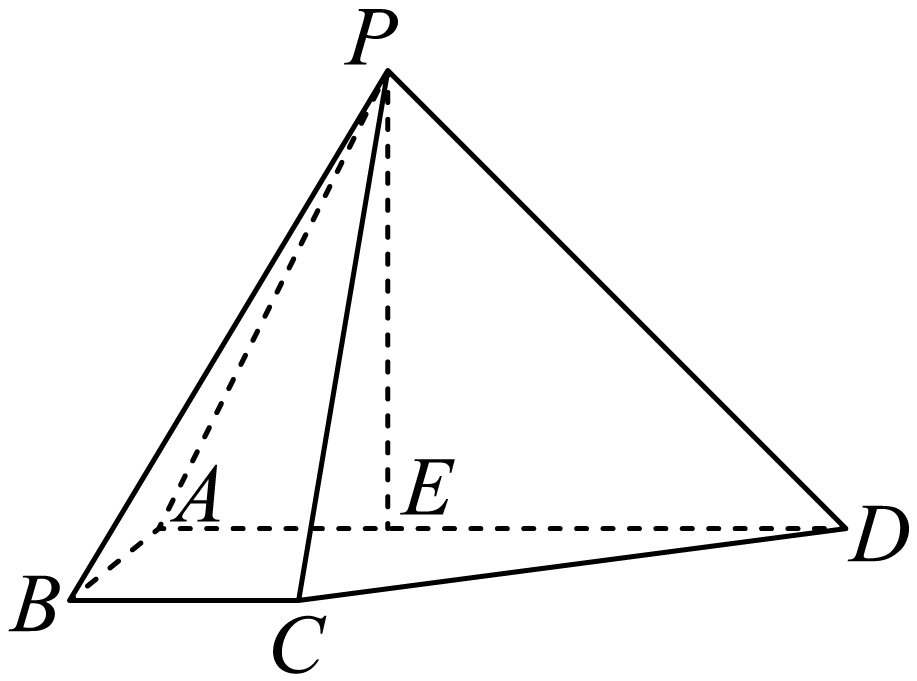
\includegraphics[width=\linewidth]{figures/2024_bj_q17.png}
\end{minipage}
\item（14分）

已知某险种的保费为 $0.4$ 万元，前 $3$ 次出险每次赔付 $0.8$ 万元，第 $4$ 次赔付 $0.6$ 万元. 在总体中抽样 $100$ 单，以频率估计概率，数据如下表：
\begin{tightcenter}
\begin{tabular}{c|ccccc}
\hline
赔偿次数 & 0 & 1 & 2 & 3 & 4\\ \hline
单数 & 800 & 100 & 60 & 30 & 10\\ \hline
\end{tabular}
\end{tightcenter}
\subq{（1）}{求随机抽取一单，赔偿不少于 $2$ 次的概率；}

\subq{（2）}{}
\subq{（i）}{毛利润是保费与赔偿金额之差. 设毛利润为 $X$，估计 $X$ 的数学期望；}

\subq{（ii）}{若未赔偿过的保单下一保险期的保费下降 $4\%$，已赔偿过的增加 $20\%$. 估计保单下一保险期毛利润的数学期望.}
\item（15分）

已知椭圆方程 $C:\dfrac{x^2}{a^2}+\dfrac{y^2}{b^2}=1(a>b>0)$，焦点和短轴端点构成边长为 $2$ 的正方形，过 $(0,t)(t>\sqrt2)$ 的直线 $l$ 与椭圆交于 $A,B$，$C(0,1)$，连接 $AC$ 交椭圆于 $D$.

\subq{（1）}{求椭圆方程和离心率；}

\subq{（2）}{若直线 $BD$ 的斜率为 $0$，求 $t$.}
\item（15分）

已知 $f(x)=x+k\ln(1+x)$，在 $(t,f(t))(t>0)$ 处切线为 $l$.

\subq{（1）}{若切线 $l$ 的斜率 $k=-1$，求 $f(x)$ 单调区间；}

\subq{（2）}{证明：切线 $l$ 不经过 $(0,0)$；}

\subq{（3）}{已知 $k=1$，$A(t,f(t))$，$C(0,f(t))$，$O(0,0)$，其中 $t>0$，切线 $l$ 与 $y$ 轴交于点 $B$ 时. 当 $2S_{\triangle ACO}=15S_{\triangle ABO}$，符合条件的 $A$ 的个数为多少？（参考数据：$1.09<\ln3<1.10$，$1.60<\ln5<1.61$，$1.94<\ln7<1.95$）}
\item（15分）

设集合 $M=\{(i,j,s,t)\mid i\in\{1,2\},j\in\{3,4\},s\in\{5,6\},t\in\{7,8\},2\mid(i+j+s+t)\}$. 对于给定有穷数列 $A:\{a_n\}(1\leq n\leq8)$，及序列 $\Omega: \omega_1,\omega_2,\cdots,\omega_s$，$\omega_k=(i_k,j_k,s_k,t_k)\in M$，定义变换 $T$：将数列 $A$ 的第 $i_1,j_1,s_1,t_1$ 项加 $1$，得到数列 $T_1(A)$；将数列 $T_1(A)$ 的第 $i_2,j_2,s_2,t_2$ 列加 $1$，得到数列 $T_2T_1(A)\cdots$；重复上述操作，得到数列 $T_s\cdots T_2T_1(A)$，记为 $\Omega(A)$.

\subq{（1）}{给定数列 $A:1,3,2,4,6,3,1,9$ 和序列 $\Omega:(1,3,5,7),(2,4,6,8),(1,3,5,7)$，写出 $\Omega(A)$；}

\subq{（2）}{是否存在序列 $\Omega$，使得 $\Omega(A)$ 为 $a_1+2,a_2+6,a_3+4,a_4+2,a_5+8,a_6+2,a_7+4,a_8+4$，若存在，写出一个符合条件的 $\Omega$；若不存在，请说明理由；}

\subq{（3）}{若数列 $A$ 的各项均为正整数，且 $a_1+a_3+a_5+a_7$ 为偶数，证明：“存在序列 $\Omega$，使得 $\Omega(A)$ 为常数列”的充要条件为 $a_1+a_2=a_3+a_4=a_5+a_6=a_7+a_8$.}
\end{examanswers}

\end{document}
